
\newpage
\begin{figure}[h]
  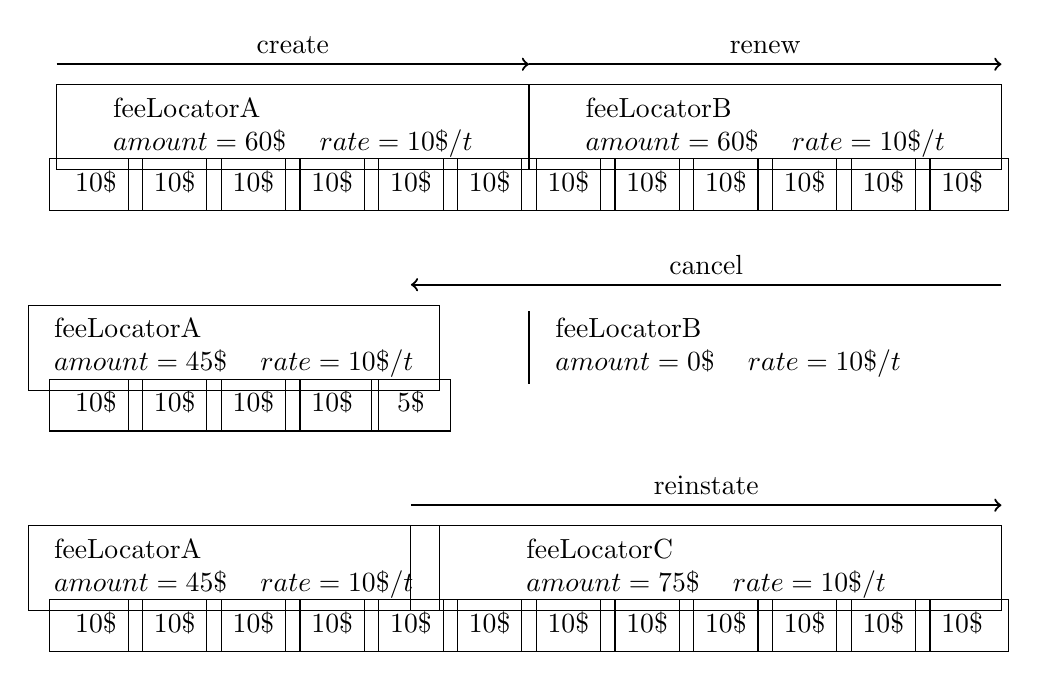
\begin{tikzpicture} [
      charge/.style={draw, rectangle, minimum width=6cm},
      schedule/.style={draw, rectangle, minimum width=1cm}
   ]
    \draw[->, thick] (-3, 0.8) -- node[above]{create} (3, 0.8);
    \draw[->, thick] (3, 0.8) -- node[above]{renew} (9, 0.8);
    \node[charge, minimum width=6cm] (ndCreate) {
      \begin{tabular}{l l}
        feeLocatorA & \\
        $amount=60\$$ & $rate=10\$/t$
      \end{tabular}
    };
    \node[charge, right of=ndCreate, node distance=6cm] (ndRenew) {
      \begin{tabular}{l l}
        feeLocatorB & \\
        $amount=60\$$ & $rate=10\$/t$
      \end{tabular}
    };
    \node[schedule, below of=ndCreate, node distance=0.73cm, xshift=-2.5cm] (c1) {
      \begin{tabular}{l}
        $10\$$
      \end{tabular}
    };
    \node[schedule, right of=c1, node distance=1cm] (c2) {
      \begin{tabular}{l}
        $10\$$
      \end{tabular}
    };
    \node[schedule, right of=c2, node distance=1cm] (c3) {
      \begin{tabular}{l}
        $10\$$
      \end{tabular}
    };
    \node[schedule, right of=c3, node distance=1cm] (c4) {
      \begin{tabular}{l}
        $10\$$
      \end{tabular}
    };
    \node[schedule, right of=c4, node distance=1cm] (c5) {
      \begin{tabular}{l}
        $10\$$
      \end{tabular}
    };
    \node[schedule, right of=c5, node distance=1cm] (c6) {
      \begin{tabular}{l}
        $10\$$
      \end{tabular}
    };
    \node[schedule, right of=c6, node distance=1cm] (c7) {
      \begin{tabular}{l}
        $10\$$
      \end{tabular}
    };
    \node[schedule, right of=c7, node distance=1cm] (c8) {
      \begin{tabular}{l}
        $10\$$
      \end{tabular}
    };
    \node[schedule, right of=c8, node distance=1cm] (c9) {
      \begin{tabular}{l}
        $10\$$
      \end{tabular}
    };
    \node[schedule, right of=c9, node distance=1cm] (c10) {
      \begin{tabular}{l}
        $10\$$
      \end{tabular}
    };
    \node[schedule, right of=c10, node distance=1cm] (c11) {
      \begin{tabular}{l}
        $10\$$
      \end{tabular}
    };
    \node[schedule, right of=c11, node distance=1cm] (c12) {
      \begin{tabular}{l}
        $10\$$
      \end{tabular}
    };

    \draw[->, thick] (9, -2) -- node[above]{cancel} (1.5, -2);
    \node[draw, rectangle, minimum width=4.5cm, below of=ndCreate, node distance=2.8cm, xshift=-0.75cm] (ndCancel) {
      \begin{tabular}{l l}
        feeLocatorA & \\
        $amount=45\$$ & $rate=10\$/t$
      \end{tabular}
    };
    \draw[-] (3, -2.34) -- node[right]{
      \begin{tabular}{l l}
        feeLocatorB & \\
        $amount=0\$$ & $rate=10\$/t$
      \end{tabular}
    } (3, -3.26);
    \node[schedule, below of=ndCancel, node distance=0.73cm, xshift=-1.75cm] (d1) {
      \begin{tabular}{l}
        $10\$$
      \end{tabular}
    };
    \node[schedule, right of=d1, node distance=1cm] (d2) {
      \begin{tabular}{l}
        $10\$$
      \end{tabular}
    };
    \node[schedule, right of=d2, node distance=1cm] (d3) {
      \begin{tabular}{l}
        $10\$$
      \end{tabular}
    };
    \node[schedule, right of=d3, node distance=1cm] (d4) {
      \begin{tabular}{l}
        $10\$$
      \end{tabular}
    };
    \node[schedule, right of=d4, node distance=1cm] (d5) {
      \begin{tabular}{l}
        $5\$$
      \end{tabular}
    };

    \draw[->, thick] (1.5, -4.8) -- node[above]{reinstate} (9, -4.8);
    \node[draw, rectangle, minimum width=4.5cm, below of=ndCancel, node distance=2.8cm] (ndReinstate1) {
      \begin{tabular}{l l}
        feeLocatorA & \\
        $amount=45\$$ & $rate=10\$/t$
      \end{tabular}
    };
    \node[draw, rectangle, minimum width=7.5cm, right of=ndReinstate1, node distance=6cm] (ndReinstate2) {
      \begin{tabular}{l l}
        feeLocatorC & \\
        $amount=75\$$ & $rate=10\$/t$
      \end{tabular}
    };
    \node[schedule, below of=ndReinstate1, node distance=0.73cm, xshift=-1.75cm] (e1) {
      \begin{tabular}{l}
        $10\$$
      \end{tabular}
    };
    \node[schedule, right of=e1, node distance=1cm] (e2) {
      \begin{tabular}{l}
        $10\$$
      \end{tabular}
    };
    \node[schedule, right of=e2, node distance=1cm] (e3) {
      \begin{tabular}{l}
        $10\$$
      \end{tabular}
    };
    \node[schedule, right of=e3, node distance=1cm] (e4) {
      \begin{tabular}{l}
        $10\$$
      \end{tabular}
    };
    \node[schedule, right of=e4, node distance=1cm] (e5) {
      \begin{tabular}{l}
        $10\$$
      \end{tabular}
    };
    \node[schedule, right of=e5, node distance=1cm] (e6) {
      \begin{tabular}{l}
        $10\$$
      \end{tabular}
    };
    \node[schedule, right of=e6, node distance=1cm] (e7) {
      \begin{tabular}{l}
        $10\$$
      \end{tabular}
    };
    \node[schedule, right of=e7, node distance=1cm] (e8) {
      \begin{tabular}{l}
        $10\$$
      \end{tabular}
    };
    \node[schedule, right of=e8, node distance=1cm] (e9) {
      \begin{tabular}{l}
        $10\$$
      \end{tabular}
    };
    \node[schedule, right of=e9, node distance=1cm] (e10) {
      \begin{tabular}{l}
        $10\$$
      \end{tabular}
    };
    \node[schedule, right of=e10, node distance=1cm] (e11) {
      \begin{tabular}{l}
        $10\$$
      \end{tabular}
    };
    \node[schedule, right of=e11, node distance=1cm] (e12) {
      \begin{tabular}{l}
        $10\$$
      \end{tabular}
    };
    
  \end{tikzpicture}
  \caption{
    Standard Socotra fixed rate fees: As the extent of the fees (top boxes) change during modifications, the
    amounts of the fees correspondingly change and fees are projected into schedules (bottom boxes) proportional
    the fee / schedule intersection. Fees that fall outside the policy range on a
    cancellation are discarded by setting their amounts to zero. On reinstatement new fees are
    created to replace the discarded fees.
  }
  \label{fig:3:1}
\end{figure}

\newpage
\begin{figure}[h]
  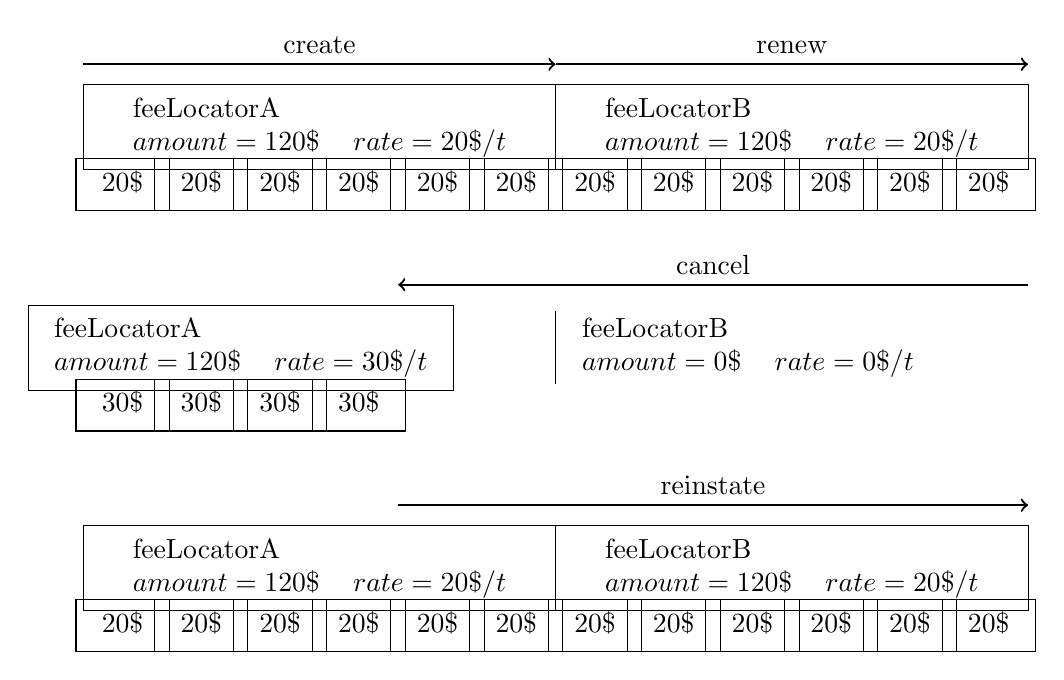
\begin{tikzpicture} [
      charge/.style={draw, rectangle, minimum width=6cm},
      schedule/.style={draw, rectangle, minimum width=1cm}
   ]
    \draw[->, thick] (-3, 0.8) -- node[above]{create} (3, 0.8);
    \draw[->, thick] (3, 0.8) -- node[above]{renew} (9, 0.8);
    \node[charge, minimum width=6cm] (ndCreate) {
      \begin{tabular}{l l}
        feeLocatorA & \\
        $amount=120\$$ & $rate=20\$/t$
      \end{tabular}
    };
    \node[charge, right of=ndCreate, node distance=6cm] (ndRenew) {
      \begin{tabular}{l l}
        feeLocatorB & \\
        $amount=120\$$ & $rate=20\$/t$
      \end{tabular}
    };
    \node[schedule, below of=ndCreate, node distance=0.73cm, xshift=-2.5cm] (c1) {
      \begin{tabular}{l}
        $20\$$
      \end{tabular}
    };
    \node[schedule, right of=c1, node distance=1cm] (c2) {
      \begin{tabular}{l}
        $20\$$
      \end{tabular}
    };
    \node[schedule, right of=c2, node distance=1cm] (c3) {
      \begin{tabular}{l}
        $20\$$
      \end{tabular}
    };
    \node[schedule, right of=c3, node distance=1cm] (c4) {
      \begin{tabular}{l}
        $20\$$
      \end{tabular}
    };
    \node[schedule, right of=c4, node distance=1cm] (c5) {
      \begin{tabular}{l}
        $20\$$
      \end{tabular}
    };
    \node[schedule, right of=c5, node distance=1cm] (c6) {
      \begin{tabular}{l}
        $20\$$
      \end{tabular}
    };
    \node[schedule, right of=c6, node distance=1cm] (c7) {
      \begin{tabular}{l}
        $20\$$
      \end{tabular}
    };
    \node[schedule, right of=c7, node distance=1cm] (c8) {
      \begin{tabular}{l}
        $20\$$
      \end{tabular}
    };
    \node[schedule, right of=c8, node distance=1cm] (c9) {
      \begin{tabular}{l}
        $20\$$
      \end{tabular}
    };
    \node[schedule, right of=c9, node distance=1cm] (c10) {
      \begin{tabular}{l}
        $20\$$
      \end{tabular}
    };
    \node[schedule, right of=c10, node distance=1cm] (c11) {
      \begin{tabular}{l}
        $20\$$
      \end{tabular}
    };
    \node[schedule, right of=c11, node distance=1cm] (c12) {
      \begin{tabular}{l}
        $20\$$
      \end{tabular}
    };

    \draw[->, thick] (9, -2) -- node[above]{cancel} (1.0, -2);
    \node[draw, rectangle, minimum width=4cm, below of=ndCreate, node distance=2.8cm, xshift=-1.0cm] (ndCancel) {
      \begin{tabular}{l l}
        feeLocatorA & \\
        $amount=120\$$ & $rate=30\$/t$
      \end{tabular}
    };
    \draw[-] (3, -2.34) -- node[right]{
      \begin{tabular}{l l}
        feeLocatorB & \\
        $amount=0\$$ & $rate=0\$/t$
      \end{tabular}
    } (3, -3.26);
    \node[schedule, below of=ndCancel, node distance=0.73cm, xshift=-1.5cm] (d1) {
      \begin{tabular}{l}
        $30\$$
      \end{tabular}
    };
    \node[schedule, right of=d1, node distance=1cm] (d2) {
      \begin{tabular}{l}
        $30\$$
      \end{tabular}
    };
    \node[schedule, right of=d2, node distance=1cm] (d3) {
      \begin{tabular}{l}
        $30\$$
      \end{tabular}
    };
    \node[schedule, right of=d3, node distance=1cm] (d4) {
      \begin{tabular}{l}
        $30\$$
      \end{tabular}
    };

    \draw[->, thick] (1.0, -4.8) -- node[above]{reinstate} (9, -4.8);
    \node[draw, rectangle, minimum width=6cm, below of=ndCancel, node distance=2.8cm, xshift=1.0cm] (ndReinstate1) {
      \begin{tabular}{l l}
        feeLocatorA & \\
        $amount=120\$$ & $rate=20\$/t$
      \end{tabular}
    };
    \node[draw, rectangle, minimum width=6cm, right of=ndReinstate1, node distance=6cm] (ndReinstate2) {
      \begin{tabular}{l l}
        feeLocatorB & \\
        $amount=120\$$ & $rate=20\$/t$
      \end{tabular}
    };
    \node[schedule, below of=ndReinstate1, node distance=0.73cm, xshift=-2.5cm] (e1) {
      \begin{tabular}{l}
        $20\$$
      \end{tabular}
    };
    \node[schedule, right of=e1, node distance=1cm] (e2) {
      \begin{tabular}{l}
        $20\$$
      \end{tabular}
    };
    \node[schedule, right of=e2, node distance=1cm] (e3) {
      \begin{tabular}{l}
        $20\$$
      \end{tabular}
    };
    \node[schedule, right of=e3, node distance=1cm] (e4) {
      \begin{tabular}{l}
        $20\$$
      \end{tabular}
    };
    \node[schedule, right of=e4, node distance=1cm] (e5) {
      \begin{tabular}{l}
        $20\$$
      \end{tabular}
    };
    \node[schedule, right of=e5, node distance=1cm] (e6) {
      \begin{tabular}{l}
        $20\$$
      \end{tabular}
    };
    \node[schedule, right of=e6, node distance=1cm] (e7) {
      \begin{tabular}{l}
        $20\$$
      \end{tabular}
    };
    \node[schedule, right of=e7, node distance=1cm] (e8) {
      \begin{tabular}{l}
        $20\$$
      \end{tabular}
    };
    \node[schedule, right of=e8, node distance=1cm] (e9) {
      \begin{tabular}{l}
        $20\$$
      \end{tabular}
    };
    \node[schedule, right of=e9, node distance=1cm] (e10) {
      \begin{tabular}{l}
        $20\$$
      \end{tabular}
    };
    \node[schedule, right of=e10, node distance=1cm] (e11) {
      \begin{tabular}{l}
        $20\$$
      \end{tabular}
    };
    \node[schedule, right of=e11, node distance=1cm] (e12) {
      \begin{tabular}{l}
        $20\$$
      \end{tabular}
    };
    
  \end{tikzpicture}
  \caption{
    Standard Socotra fixed amount fees: As the extent of the fees (top boxes) change during modifications, the
    amounts of the fees stay fixed and fees are projected into schedules (bottom boxes) proportional
    the fee / schedule intersection. Fees that fall outside the policy range on a
    cancellation are discarded by setting their amounts to zero. On reinstatement discarded fees are
    reextened.
  }
  \label{fig:3:2}
\end{figure}
